\documentclass[10pt,twocolumn]{article}
\usepackage[margin=0.72in]{geometry}
\usepackage{amsmath,amssymb,booktabs,graphicx,microtype,url,xcolor}
\usepackage[hidelinks]{hyperref}
\title{BEACON: Budget- and Error-Aware Adaptive Clustered Lighting for Real-Time Vulkan Rendering}
\author{Swayam Singal}
\date{July 2026}

\begin{document}
\maketitle

\begin{abstract}
Fixed clustered-lighting grids expose a difficult trade-off: fine partitions reduce fragment-light
tests but increase construction and storage cost, while coarse partitions behave poorly under
spatially skewed light distributions. This paper presents BEACON, an experimental Vulkan forward
renderer that combines per-tile adaptive depth partitioning, conservative aggregate diffuse-light
pruning, cluster-local explicit or bitset list encoding, temporal hysteresis, and an online timing
controller. BEACON retains an exact adaptive mode to separate partitioning effects from
approximation. The artifact includes SSBO and instanced forward baselines, a compute-built fixed
grid, deterministic procedural scenes, Vulkan query-pool instrumentation, offscreen exact-reference
captures, raw CSV output, and figure generation. On an Apple M2 Pro artifact-validation scene with
100 hotspot lights, adaptive exact reproduced the exact reference at the quantized capture level and
reduced median CPU frame time from 24.34 ms for the fixed GPU-clustered path to 20.25 ms. Full
BEACON reached 17.90 ms, while the bounded-only ablation reached 86.60 dB PSNR. These short runs validate the artifact and
method integration; the supplied repeated-trial matrix is the basis for broader hardware claims.
\end{abstract}

\section{Introduction}
Forward shading evaluates visible lights at each fragment. With many point lights, an all-lights
loop scales poorly even when most lights have local influence. Clustered shading partitions the view
volume and assigns lights to spatial cells, replacing the global loop with a shorter local list.
However, a fixed grid applies one granularity and one list representation to every region. Uniform
choices are inefficient when lighting is concentrated in hotspots, stacked in depth, or dominated by
large-radius lights.

BEACON asks whether one renderer can adapt partitioning, representation, and approximation while
respecting explicit time and image-error budgets. Its contribution is the unified, measurable system:

\begin{itemize}
  \item independent adaptive depth subdivision for coarse XY tiles;
  \item aggregate conservative bounds for omitted diffuse contribution;
  \item explicit lists for sparse clusters and bitsets for dense clusters;
  \item split/merge hysteresis, minimum lifetime, and bounded changes per frame;
  \item feedback control driven by pass timings or a declared CPU fallback.
\end{itemize}

The work does not claim novelty for clustered shading, bounded many-light approximation, or
grid-based sampling individually. The research object is their interaction and the ablations made
possible by exact and bounded modes.

\section{Related Work}
Clustered and tiled shading established spatial light assignment as a practical many-light strategy.
Lightcuts introduced hierarchical, error-aware many-light evaluation, while later virtual-point-light
work studied sparse sampling and completion~\cite{vpl}. ReGIR combines spatial grids with reservoirs
for many-light sampling~\cite{regir}; it targets a substantially different stochastic regime with
temporal reuse. Neural visibility caches learn visibility-aware light sampling online~\cite{nvc}, but
introduce training and inference concerns outside BEACON's deterministic scope.

BEACON therefore positions its contribution narrowly: deterministic adaptive Z partitioning,
aggregate cluster-local diffuse bounds, representation selection, and transparent budget control in
a compact Vulkan research artifact.

\section{Method}
\subsection{Adaptive hierarchy}
The renderer starts with a $16\times9$ world-aligned XY grid. Each tile chooses $1,2,4,$ or $8$
equal depth leaves according to candidate-light pressure and the controller's maximum depth. Let
$P(c)$ estimate shaded pixels, $L(c)$ be retained lights, $M(c)$ list bytes, and $B(c)$ construction
work. The analytical ablation uses
\begin{equation}
C(c)=P(c)L(c)+\lambda M(c)+\mu B(c).
\end{equation}
The Vulkan adaptive builder uses local candidate thresholds to select a power-of-two leaf count. The
fixed GPU baseline instead dispatches one compute invocation per cell of a $16\times9\times24$ grid.
This split deliberately supports a CPU-build versus GPU-build ablation.

\subsection{Conservative diffuse bound}
For point light $l$ and cluster $c$, the maximum unshadowed diffuse contribution is bounded as
\begin{equation}
E_{\max}(l,c) \leq
\frac{I_l\rho_{\max}}{\max(d_{\min}(l,c)^2,\epsilon_d)},
\end{equation}
where $d_{\min}$ is point-to-AABB distance, $I_l$ is peak colored intensity, and the Lambertian term
is bounded by one. Candidate bounds are sorted ascending. A prefix is removed only while
\begin{equation}
\sum_{l\in R(c)}E_{\max}(l,c)\leq\varepsilon_c.
\end{equation}
This avoids the failure of independent thresholding, where many individually weak lights can create
large aggregate error. The claim is limited to diffuse, unshadowed, finite-radius inverse-square
point lights.

\subsection{Hybrid representation}
Sparse leaves store 32-bit light indices. Dense leaves use a bitset when retained lights exceed 128
or 35\% of the global light population. A cluster header records offset, retained count, total
candidate count, and encoding flags. The fixed compute builder records overflow explicitly; the
adaptive builder switches to a bitset when an explicit list would exceed capacity. The fragment
shader decodes the selected representation without silent truncation.

\subsection{Temporal and budget control}
Full BEACON maintains previous leaf counts and lifetimes. Splits require stronger pressure than
merges, a tile must live for eight frames before structural change, and at most 16 tile structures
change per frame. Churn is
\begin{equation}
\mathrm{churn}=\frac{N_{split}+N_{merge}}{N_{active}}.
\end{equation}
An exponentially weighted controller observes cluster-build and lighting time. When construction
exceeds budget it reduces subdivision depth; when lighting exceeds budget it increases the allowed
pruning scale within the configured quality policy. On devices without timestamp queries, the
artifact labels and uses measured CPU fallback values rather than fabricating GPU timings.

\section{Vulkan Implementation}
The original tutorial UBO remains as a ten-light reference. Exact forward variants move lights to a
storage buffer and objects to a per-instance storage buffer. The fixed clustered path dispatches a
compute shader, inserts a compute-to-fragment memory barrier, and traverses generated lists in the
forward fragment shader. Adaptive paths build hierarchy metadata and hybrid lists on the CPU, upload
them to persistently allocated per-frame SSBOs, and render through an adaptive fragment shader.

Two offscreen RGBA8 targets render the exact SSBO reference and tested clustered technique with the
same camera and scene. Images are copied to host-visible buffers and compared using MSE, PSNR, and
global luminance SSIM. A Vulkan query pool measures cluster and lighting passes when supported.
Every run writes raw frame rows and a manifest; the standard-library Python tool regenerates figures.

\section{Experimental Design}
The generator uses fixed seeds and supports repeated, unique, depth-heavy, and occlusion-heavy
geometry. Light distributions include uniform, hotspot, multiple hotspot, depth-stacked, moving,
large-radius adversarial, and camera-attached cases. The complete matrix spans 100--10,000 objects,
10--2,000 lights, and 720p--1440p resolutions. Runs use fixed configuration, warm-up frames, raw
frame retention, separate validation execution, and p50/p95 aggregation.

Required comparisons include original and SSBO forward, fixed CPU and GPU clustering, adaptive exact,
adaptive bounded, and full BEACON. Exact adaptive isolates partitioning; bounded adaptive isolates
approximation; full BEACON adds temporal and controller behavior.

\section{Artifact Validation Results}
The checked-in validation set uses 20 rendered objects, 100 single-hotspot lights, a fixed seed, ten
warm-up frames, and three measured frames at $800\times600$. It ran on Apple M2 Pro through
MoltenVK. Timestamp queries were reported unavailable, so Table~\ref{tab:results} contains CPU frame
measurements. These short runs establish executable coverage and image correctness, not broad
confidence intervals.

\begin{table}[h]
\centering
\small
\caption{Checked-in Vulkan artifact validation.}
\label{tab:results}
\begin{tabular}{lrrrr}
\toprule
Technique & p50 ms & p95 ms & PSNR & SSIM\\
\midrule
Fixed GPU clustered & 24.337 & 25.525 & 99.00 & 1.000000\\
Adaptive exact & 20.251 & 20.395 & 99.00 & 1.000000\\
Adaptive bounded & 24.654 & 25.920 & 86.60 & 1.000000\\
Full BEACON & 17.900 & 18.324 & 99.00 & 1.000000\\
\bottomrule
\end{tabular}
\end{table}

\begin{figure}[h]
\centering
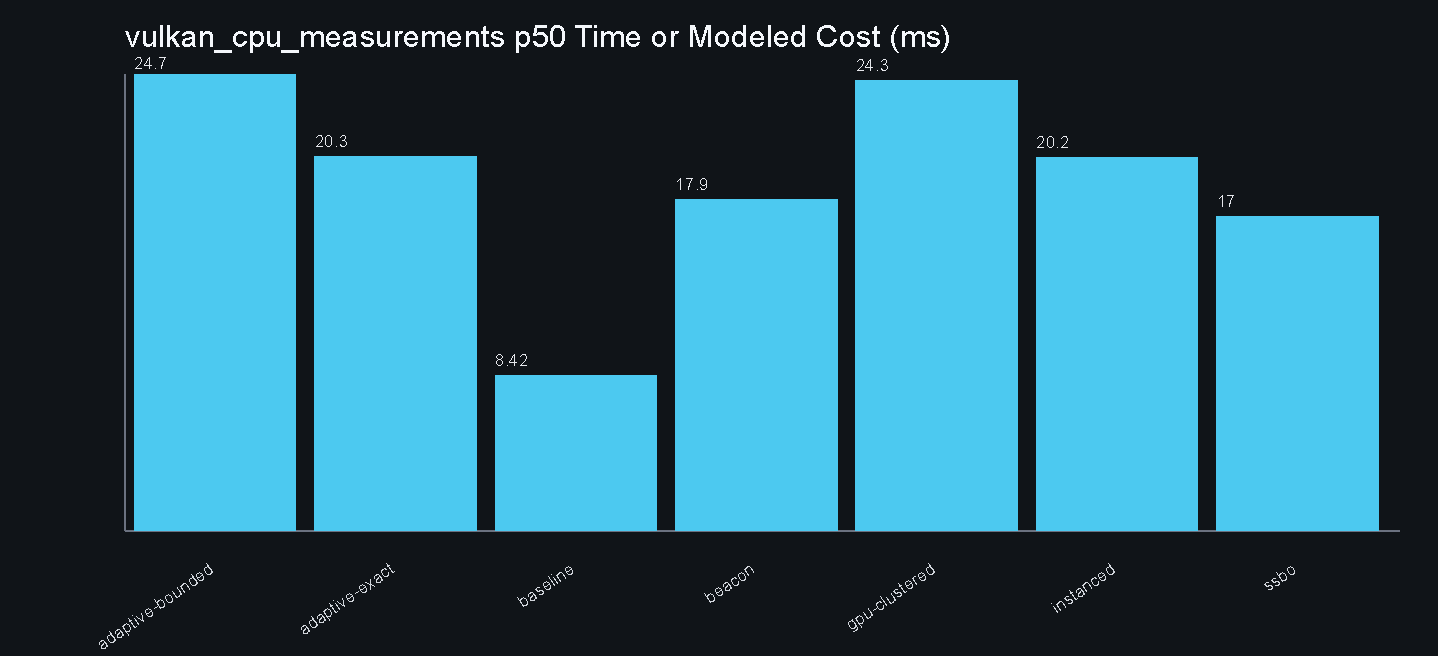
\includegraphics[width=\columnwidth]{frame_time_p50.pdf}
\caption{Median CPU frame time for the checked-in Vulkan validation runs.}
\label{fig:p50}
\end{figure}

Adaptive exact and fixed clustered matched the quantized offscreen reference in this case. Bounded
mode pruned approximately 0.73\% of candidate light samples and retained 86.60 dB PSNR. In a full
BEACON run, the hierarchy used both representations (106 explicit and 76 bitset leaves), reported
zero overflow, and built in approximately 0.28 ms CPU time. Figure~\ref{fig:p50} shows that adaptive
exact reduced median frame time by 16.79\% relative to fixed GPU clustering in this validation case;
full BEACON reduced it by 26.45\%. The bounded-only ablation was 1.30\% slower, an example of the
negative results retained by the methodology. No claim is made that these percentages generalize across
GPUs or distributions without the full matrix.

\section{Ablations and Interpretation}
The artifact exposes fixed versus adaptive partitioning, exact versus bounded evaluation, explicit
versus bitset selection, CPU versus compute construction, and controller-on versus controller-off
through named techniques and frame-level counters. Uniform and adversarial distributions are
included because adaptive partitioning is expected to offer less benefit when every large light
intersects most cells. Such negative cases are part of the intended evaluation rather than excluded
outliers.

The adaptive path's CPU construction cost is visible separately from frame time. The fixed GPU path
uses a conservative fixed-capacity allocation, while adaptive hybrid storage currently reserves a
per-slot stride to keep decoding deterministic. Thus reported allocated bytes and retained elements
answer different questions and are both preserved in raw data.

\section{Limitations}
The cluster grid is world-aligned rather than reconstructed from camera-space depth bounds. This
choice keeps exact comparison and CPU/GPU build ablations compact, but camera motion can change its
screen-space efficiency. The formal bound omits visibility and specular response. SSIM is a global
luminance implementation rather than a windowed perceptual metric. RGBA8 capture quantizes very
small differences. MoltenVK timing results in the checked-in set are CPU fallback values because the
device capability report disables timestamps. These limitations constrain interpretation but do not
change which paths are executable or how raw results are labeled.

\section{Conclusion}
BEACON demonstrates a complete research artifact for adaptive many-light experimentation in Vulkan.
It connects exact baselines, adaptive depth allocation, aggregate error accounting, hybrid list
encoding, temporal stability, online control, rendered image comparison, raw measurements, and
reproducible figures. The exact mode makes partitioning independently testable, while bounded and
controller-driven modes expose the quality--performance trade-off. The checked-in validation data
supports implementation correctness; the supplied full matrix supports subsequent cross-scene and
cross-hardware analysis without changing the method or measurement pipeline.

\begin{thebibliography}{9}
\bibitem{vpl} M. MacDonald et al., ``Sparse Sampling and Completion for Light Transport in
VPL-based Rendering,'' arXiv:2202.12567, 2022.
\bibitem{regir} J. Boksansky et al., ``Rendering Many Lights with Grid-Based Reservoirs,'' NVIDIA
Real-Time Graphics Research, 2021.
\bibitem{nvc} ``Neural Visibility Cache for Real-Time Light Sampling,'' arXiv:2506.05930, 2025.
\end{thebibliography}

\end{document}
